\documentclass[tikz,border=8pt]{standalone}
\usepackage{amsmath}
\usetikzlibrary{arrows.meta,decorations.pathmorphing}
\definecolor{ink}{HTML}{17324D}
\definecolor{accent}{HTML}{0F766E}
\definecolor{gold}{HTML}{C28524}
\begin{document}
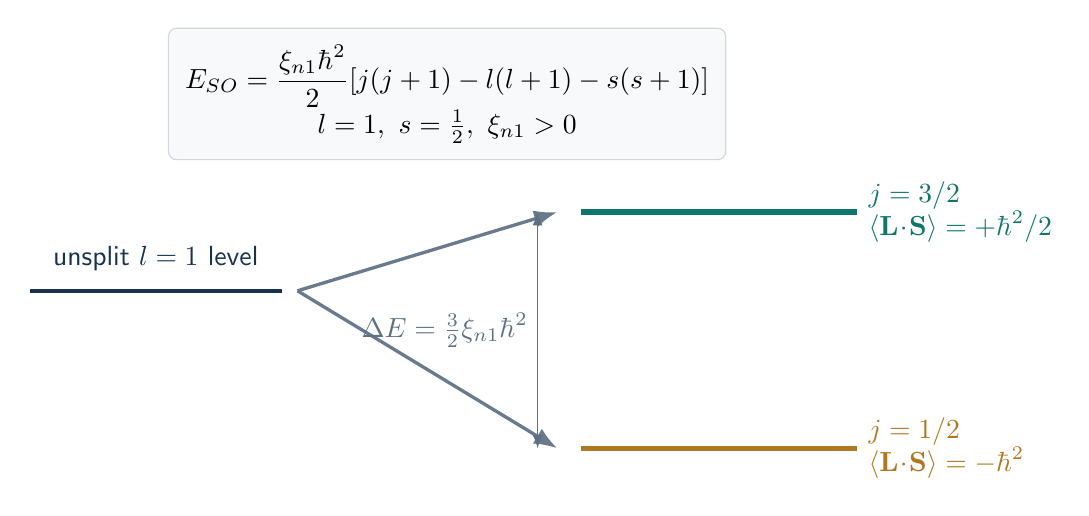
\begin{tikzpicture}[font=\sffamily,>=Latex]
 \def\scaleE{2.0}
 \def\etop{0.5}
 \def\ebottom{-1.0}
 \draw[ink,line width=1.5pt] (0,0)--(3.2,0)
   node[midway,above=3pt] {unsplit $l=1$ level};
 \draw[accent,line width=2pt] (7,{\scaleE*\etop})--(10.5,{\scaleE*\etop})
   node[right,align=left] {$j=3/2$\\$\langle\mathbf L\!\cdot\!\mathbf S\rangle=+\hbar^2/2$};
 \draw[gold!90!black,line width=2pt] (7,{\scaleE*\ebottom})--(10.5,{\scaleE*\ebottom})
   node[right,align=left] {$j=1/2$\\$\langle\mathbf L\!\cdot\!\mathbf S\rangle=-\hbar^2$};
 \draw[->,ink!65,line width=1.2pt] (3.4,0)--(6.7,{\scaleE*\etop});
 \draw[->,ink!65,line width=1.2pt] (3.4,0)--(6.7,{\scaleE*\ebottom});
 \draw[<->,ink!70] (6.45,{\scaleE*\ebottom})--(6.45,{\scaleE*\etop})
   node[midway,left] {$\Delta E=\frac32\xi_{n1}\hbar^2$};
 \node[draw=ink!20,rounded corners=3pt,fill=ink!3,inner sep=6pt,align=center]
   at (5.3,2.5)
   {$\displaystyle E_{SO}=\frac{\xi_{n1}\hbar^2}{2}
   [j(j+1)-l(l+1)-s(s+1)]$\\
    $l=1,\ s=\tfrac12,\ \xi_{n1}>0$};
\end{tikzpicture}
\end{document}
